\title[Learned initialization for variational quantum circuits in HEP]{Learned initialization for variational quantum circuits on lattice and field-theory Hamiltonians: a ten-system benchmark of Q-MAML}

\author*[1]{\fnm{Arnav} \sur{Kapoor}}\email{arnavkapoor23@iiserb.ac.in}

\affil*[1]{\orgdiv{Department of Computer Science}, \orgname{Indian Institute of Science Education and Research Bhopal}, \orgaddress{\city{Bhopal}, \postcode{462066}, \state{Madhya Pradesh}, \country{India}}}

\abstract{Variational quantum algorithms are a leading route to simulating lattice field theories on near-term devices, but much of their cost is spent escaping poor parameter initializations. Q-MAML trains a classical network to predict circuit parameters across a family of Hamiltonians, yet has only been validated on spin chains and small molecules. We provide a from-scratch reimplementation that reproduces the original paper's convergence gains (15--20$\times$ fewer iterations on H$_2$) and benchmark it on high-energy-physics (HEP) classification and on ten lattice and field-theory Hamiltonians, each verified before use and replicated over three seeds. Q-MAML attains the highest HIGGS classification accuracy at every qubit count tested. On the Hamiltonians the advantage is conditional: consistent wins on two of ten systems, seed-dependent wins on two, ties on four, a tie-to-slight-loss on one, and a loss on penalty-enforced $\mathbb{Z}_2$ gauge theory. That loss is an ansatz artifact: with a structurally gauge-invariant ansatz Q-MAML is the best scheme at all three seeds. At larger sizes, Q-MAML's failures trace to pretraining converging to poor local minima of the meta-objective, visible in the training loss without test data, and restarting from the lowest-loss of several Learner initializations recovers a win. A quantum-Fisher-information probe shows Q-MAML initializations sit at higher effective dimension than random ones (0.93--0.96 versus 0.68--0.74, 4--12 qubits), consistent with a benefit from placement in parameter space rather than resistance to barren plateaus.}

\keywords{variational quantum eigensolver, meta-learning, barren plateaus, lattice gauge theory, high-energy physics, quantum machine learning}

\maketitle

%% =====================================================================================
\section{Introduction}\label{sec:intro}

Simulating lattice field theories is a flagship application for quantum computers, and the variational quantum eigensolver (VQE) is the workhorse for near-term ground-state preparation. Its cost is the number of circuit evaluations, and a large share is spent escaping poor initial parameters: random initializations are prone to barren plateaus~\cite{mcclean2018barren,cerezo2021costfunction}, and the initialization heuristics proposed to avoid them, such as near-identity blocks~\cite{grant2019initialization}, Gaussian~\cite{zhang2022escaping} or reduced-domain~\cite{wang2023trainability} sampling, are independent of the Hamiltonian being solved.

A complementary idea is to \emph{learn} the initialization. Meta-VQE~\cite{cerveralierta2021metavqe} learns energy profiles of parameterized Hamiltonians; Q-MAML~\cite{leeqmaml2025} trains a classical ``Learner'' network that maps a task descriptor (the Hamiltonian's parameters) directly to circuit angles, by back-propagating the energy through the circuit with no inner adaptation loop; recent work generates initial parameters with graph networks~\cite{qracle2025} or diffusion models~\cite{diffq2025}. Q-MAML was validated on Heisenberg chains and small molecules only, and whether it helps on the Hamiltonians and datasets of high-energy physics (HEP) is open.

We make three contributions. \textbf{(i)} We implement Q-MAML from the published algorithm and validate it against the original paper's own settings before using it on anything new, alongside a first-order variant with a truncated inner loop and a stop-gradient update as a further classification baseline. \textbf{(ii)} We benchmark it on HEP classification and on ten lattice and field-theory Hamiltonians, spanning Abelian and non-Abelian gauge theories, scalar and fermion--boson field theories, supersymmetric quantum mechanics, nuclei and neutrinos; every Hamiltonian is verified against exact limits before use and every comparison is replicated over three seeds. \textbf{(iii)} We show that the outcome is conditional on ansatz structure and system size, diagnose two of the mechanisms, and give a diagnostic that flags a failing initialization from the training loss alone. Code, results and notebooks are public (Data and code availability).

%% =====================================================================================
\section{Methods}\label{sec:methods}

\subsection{Q-MAML}\label{sec:qmaml}

A \emph{task} is a Hamiltonian $H_\phi$ with descriptor $\phi\in\mathbb{R}^d$ (masses, couplings, a discrete label). A parameterized circuit $U(\theta)$ on $n$ qubits prepares $|\psi(\theta)\rangle$ and the task cost is $\ell_\phi(\theta)=\langle\psi(\theta)|H_\phi|\psi(\theta)\rangle$. Q-MAML (Fig.~\ref{fig:framework}, Algorithm~\ref{alg:qmaml}) has two phases. \emph{Pretraining} fits a Learner $h_W$, a two-layer MLP (width 256, double precision), so that $\theta_0=s\,h_W(\phi)$ ($s=0.3$) has low energy on training tasks, by minimizing $\sum_i\ell_{\phi_i}(\theta_0^{(i)})$ over $W$ with Adam. Gradients flow through the circuit (adjoint or back-propagation) and there is no inner loop. \emph{Adaptation} freezes $W$ and, on a held-out task, runs gradient descent on $\ell_{\phi^\star}$ starting at $\theta_0=s\,h_W(\phi^\star)$. Any initializer can replace the Learner in the second phase, so the comparison isolates initialization quality.

\begin{figure}[!htb]
\centering
\resizebox{\textwidth}{!}{%
\begin{tikzpicture}[
  box/.style={draw=black!70, rounded corners=1.5pt, align=center, font=\footnotesize, inner sep=3pt,
              minimum height=9mm, minimum width=24mm, line width=0.5pt, fill=white},
  learner/.style={box, draw=qorange, fill=qorange!14},
  circuit/.style={box, draw=qblue, fill=qblue!12},
  base/.style={box, draw=black!45, fill=black!5},
  arr/.style={-{Stealth[length=2mm,width=1.6mm]}, line width=0.55pt, black!75},
  back/.style={-{Stealth[length=2mm,width=1.6mm]}, line width=0.7pt, dashed, red!65!black},
  lab/.style={font=\scriptsize, align=center}]
% ------------------------------------------------------------------ (a) pretraining
\node[font=\bfseries\large] at (-1.7,1.05) {a};
\node[lab, anchor=west] at (-1.2,1.05) {\textbf{Pretraining} (Algorithm 1): learn to map a task to good angles};
\node[box]     (a1) at (0,0)    {Task descriptor\\ $\phi_i$};
\node[learner] (a2) at (4.0,0)  {Learner\\ $h_W$ (MLP)};
\node[box]     (a3) at (8.2,0)  {Initial angles\\ $\theta_0=s\,h_W(\phi_i)$};
\node[circuit] (a4) at (12.4,0) {Circuit\\ $U(\theta_0)|0\rangle$};
\node[box]     (a5) at (16.4,0) {Energy\\ $E_i=\langle H_{\phi_i}\rangle$};
\node[box]     (al) at (16.4,-2.0) {Loss $\sum_i E_i$};
\draw[arr] (a1) -- (a2); \draw[arr] (a2) -- (a3); \draw[arr] (a3) -- (a4); \draw[arr] (a4) -- (a5);
\draw[arr] (a5) -- (al);
\draw[back] (al.west) -- (4.0,-2.0) -- (a2.south);
\node[lab, text=red!65!black] at (10.2,-1.65) {gradient $\nabla_W$ flows through the circuit; no inner loop};
% ------------------------------------------------------------------ separator
\draw[black!30, line width=0.4pt] (-1.7,-3.05) -- (18.4,-3.05);
% ------------------------------------------------------------------ (b) adaptation
\node[font=\bfseries\large] at (-1.7,-3.55) {b};
\node[lab, anchor=west] at (-1.2,-3.55) {\textbf{Adaptation} (Algorithm 2): a standard VQE loop from the predicted start};
\node[box]     (b1) at (0,-5.0)   {New task\\ $\phi^\star$};
\node[learner] (b2) at (4.0,-4.55){Learner $h_{W^\star}$\\ (frozen)};
\node[base]    (b2b) at (4.0,-6.05){Classical baselines:\\ Zero, $\pi$, Uniform, Gaussian};
\node[box]     (b3) at (8.2,-5.0) {Start point\\ $\theta_0$};
\node[circuit] (b4) at (12.4,-5.0){Circuit\\ $U(\theta)|0\rangle$};
\node[box]     (b5) at (16.4,-5.0){Energy\\ $E(\theta)$};
\node[box]     (bo) at (12.4,-7.0){Optimizer\\ $\theta\leftarrow\theta-\eta'\nabla E$};
\node[box]     (bf) at (6.9,-7.0) {Adapted state\\ $E_T\approx E_0$};
\draw[arr] (b1.east) -- ++(0.6,0) |- (b2.west); \draw[arr] (b1.east) -- ++(0.6,0) |- (b2b.west);
\draw[arr] (b2) -- (b3); \draw[arr] (b2b.east) -| (b3.south);
\draw[arr] (b3) -- (b4); \draw[arr] (b4) -- (b5);
\draw[arr] (b5.south) |- (bo.east);
\draw[arr] (bo.north) -- (b4.south);
\draw[arr] (bo.west) -- (bf.east);
\node[lab] at (14.4,-6.35) {$T$ iterations};
\end{tikzpicture}}

\caption{\textbf{The Q-MAML framework.} \textbf{a}, Pretraining (Algorithm 1): a Learner network maps each training task's descriptor to initial circuit angles; the energy is back-propagated through the circuit (dashed red path) to update the Learner, with no inner loop. \textbf{b}, Adaptation (Algorithm 2) on a held-out task: the frozen Learner (or a classical baseline) supplies $\theta_0$, and a standard VQE loop refines it. All initializers share the same adaptation phase.}
\label{fig:framework}
\end{figure}

\begin{algorithm}[t]
\caption{Q-MAML pretraining and adaptation}\label{alg:qmaml}
\begin{algorithmic}[1]
\Require task distribution $p(T)$, ansatz $U(\theta)$, Learner $h_W$, scale $s$, learning rates $\eta,\eta'$
\Statex \textbf{Pretraining (Algorithm 1)}
\For{each epoch}
  \For{each training task $T_i\sim p(T)$}
    \State $\theta_0^{(i)}\gets s\,h_W(\phi_i)$; \quad $E_i\gets\langle\psi(\theta_0^{(i)})|H_i|\psi(\theta_0^{(i)})\rangle$
    \State $W\gets W-\eta\,\nabla_W E_i$ \Comment{through the circuit; no inner loop}
  \EndFor
\EndFor
\Statex \textbf{Adaptation (Algorithm 2) on a held-out task $T^\star$}
\State $\theta\gets s\,h_{W}(\phi^\star)$
\For{$t=1,\dots,T$} $\theta\gets\theta-\eta'\,\nabla_\theta\,\ell_{\phi^\star}(\theta)$ \EndFor
\end{algorithmic}
\end{algorithm}

\paragraph{Baselines.} All baselines feed the same adaptation phase: Zero ($\theta=0$), $\pi$ ($\theta=\pi$), Uniform ($\theta\sim\mathcal{U}[-\alpha\pi,\alpha\pi]$, $\alpha=0.05$) and Gaussian ($\theta\sim\mathcal{N}(0,\gamma^2)$, $\gamma^2=1/(4S(L{+}2))$, $S=2$, $L$ layers)~\cite{zhang2022escaping}. For classification we add a first-order MAML variant: several inner gradient steps on the circuit parameters on each support set, followed by a query loss evaluated at $w_0+\mathrm{sg}(w_T-w_0)$, where $\mathrm{sg}$ is the stop-gradient operator and $w_T$ the parameters after $T$ inner steps. It shares the Learner-free circuit and head of the other classification arms, so it separates the effect of the outer-loop objective from that of the architecture.

\subsection{Benchmarks}\label{sec:bench}

\paragraph{Classification.} HIGGS (tabular features, 180\,000-event subsample~\cite{baldi2014higgs}) with tasks defined as quantile bins of the reconstructed $m_{bb}$ (six bins, 8 support and 8 query events per task, 18 training and 12 test tasks); a hybrid model (feature encoder, parameterized circuit, linear head), depth 2, ten epochs, 4/6/8 qubits. A second dataset, quark--gluon jet tagging, is run at six qubits.

\paragraph{Hamiltonians.} Fig.~\ref{fig:systems} and Table~\ref{tab:systems} list the ten systems. Each has its own module with exact diagonalization, a task sampler and a verification routine (Hermiticity; exact analytic limits such as the harmonic-oscillator spectrum, the $V{=}0$ limit or the su(2) algebra; symmetry commutation, e.g.\ $[H,G_l]=0$ and $G_l^2=\mathbb{1}$ for the $\mathbb{Z}_2$ Gauss operators; and, for $\mathbb{D}_8$, a representation-theory check over all 64 group-element pairs that caught a real bug before any run). Two systems needed a stated change of question: the neutrino and Yukawa sources study real-time dynamics, so we ask for the ground state of the same Hamiltonian instead.

\begin{figure}[!htb]
\centering
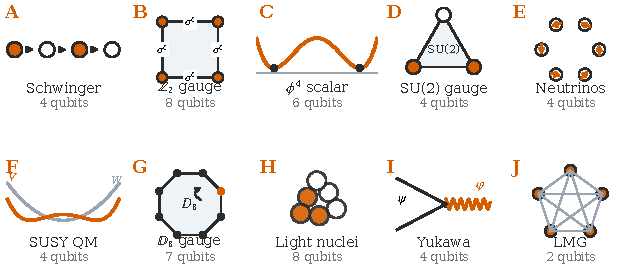
\includegraphics[width=\textwidth]{figures/fig_systems.pdf}
\caption{\textbf{The ten benchmark Hamiltonians.} Track letters as in Table~\ref{tab:systems}; qubit counts are the base sizes.}
\label{fig:systems}
\end{figure}

\begin{table}[!htb]
\caption{\textbf{The ten benchmark Hamiltonians.} HEA: hardware-efficient ansatz; HVA: Hamiltonian-variational ansatz; UCCSD: unitary coupled-cluster singles and doubles. Qubits in parentheses are the larger sizes run as extensions.}\label{tab:systems}
\begin{tabular*}{\textwidth}{@{\extracolsep\fill}llccl@{}}
\toprule
Track & System (source) & Qubits & Ansatz & Task parameters \\
\midrule
A & Lattice Schwinger model, 1+1D QED~\cite{schwingertrappedion2025} & 4 (6, 8) & HEA & $(m_0,g)$ \\
B & Single-plaquette $\mathbb{Z}_2$ LGT~\cite{z2lgtbp2025} & 8 & HEA / HVA & $(J,m,\mu)$ \\
C & $\phi^4$ scalar field~\cite{scalarfield2023} & 6 & HEA & $(m_0^2,\lambda_0)$ \\
D & SU(2) LGT, gauge field eliminated~\cite{su2hadrons2021} & 4 (6, 8) & HEA & $(\tilde m,x)$ \\
E & Collective neutrino oscillations~\cite{neutrinoqc2021,duanfullerqian2010} & 4 (6) & HEA & $(\theta,\mu)$ \\
F & Supersymmetric quantum mechanics~\cite{susyqm2026} & 4 & HEA & (superpotential, $m,g,\mu$) \\
G & Non-Abelian $\mathbb{D}_8$ LGT~\cite{d8lgt2025} & 7 & HEA & $(M,\lambda_E,\epsilon)$ \\
H & Light nuclei, lattice pionless EFT~\cite{nucleareft2026} & 8 & UCCSD & (nucleus, $t,C,D$) \\
I & Scalar Yukawa coupling~\cite{yukawa2022} & 4 & HEA & $(\eta,m)$ \\
J & Lipkin--Meshkov--Glick model~\cite{hlvqe2023} & 2 (3) & HEA & $(\epsilon,V)$ \\
\botrule
\end{tabular*}
\end{table}

\subsection{Protocol and metrics}\label{sec:protocol}

For each system, 16 training and 6 held-out tasks are drawn from the descriptor range with disjoint random seeds (held-out \emph{interpolation}); the Learner is pretrained for 40 epochs and each scheme is adapted on each held-out task for 150--300 Adam iterations. We report the final relative energy error $\varepsilon=\exp\langle\log|E_T-E_0|\rangle_{\rm tasks}/\langle|E_0|\rangle_{\rm tasks}$ against the exact ground energy $E_0$, or the log-gap $\log|E_T-E_0|$ where $E_0\approx0$ (supersymmetric quantum mechanics). Every comparison is repeated for three seeds, which change the training and test tasks, the Learner initialization and the baselines' random draws. A seed is scored as a Q-MAML \emph{win} or \emph{loss} if its error is more than 10\% below or above the best classical scheme at that seed, and a \emph{tie} otherwise, including when both errors are below $10^{-6}$ (the floor set by the $10^{-8}$ regularizer in the log-gap). Classification uses Welch's $t$-test and Cohen's $d=(\bar x_1-\bar x_2)/s_p$ with $s_p=\sqrt{(s_1^2+s_2^2)/2}$, uncorrected for multiple comparisons unless stated.

%% =====================================================================================
\section{Results}\label{sec:results}

\subsection{Validation against the original paper}\label{sec:validation}

Before extending Q-MAML we checked that our implementation reproduces the original paper's own settings (Fig.~\ref{fig:calibration}). On the H$_2$ molecule, with the paper's exact circuit (4 qubits, depth 7, 2000 iterations), Q-MAML reaches machine precision by iteration $\sim$100 whereas classical initializations need 1500--2000, a 15--20$\times$ reduction in circuit evaluations, and all non-degenerate schemes converge to the same final energy. On the Heisenberg XYZ chain (6 qubits; the paper's circuit is not available to us, so the ansatz is reconstructed) the gain is 4--6$\times$. In both, the advantage is convergence speed from a better starting point, not a different optimum.

\begin{figure}[!htb]
\centering
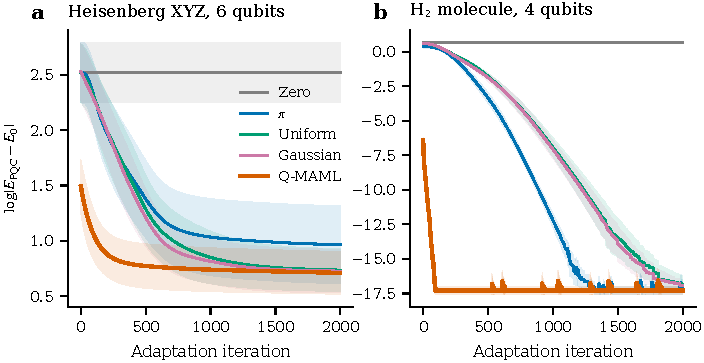
\includegraphics[width=\textwidth]{figures/fig_calibration.pdf}
\caption{\textbf{Validation on the original paper's settings.} Mean log-gap over held-out tasks (bands: half a standard deviation) versus adaptation iteration for \textbf{a}, the Heisenberg XYZ chain (reconstructed ansatz) and \textbf{b}, the H$_2$ molecule (exact ansatz). Q-MAML starts closer to the ground state and converges 4--6$\times$ and 15--20$\times$ faster, respectively.}
\label{fig:calibration}
\end{figure}

\subsection{HEP classification}\label{sec:class}

On HIGGS, Q-MAML has the highest mean validation accuracy at every qubit count, over 8 seeds each (Fig.~\ref{fig:higgs}, Table~\ref{tab:higgs}). Table~\ref{tab:higgs} gives the tests against Gaussian initialization and against the post-hoc best classical scheme; the margin against Gaussian is significant at every qubit count ($p<0.01$, $d>2.0$), and against the best classical scheme it is significant at 4 and 6 qubits ($p<0.02$, $d>1.5$) and directional at 8 ($p=0.081$, $d=0.96$). Q-MAML is also the only variant whose training meta-loss decreases appreciably. On quark--gluon tagging (six qubits, two seeds) the gap is larger, $0.776\pm0.005$ against $0.594$--$0.599$ for the classical schemes, but two seeds is directional evidence only.

\begin{figure}[!htb]
\centering
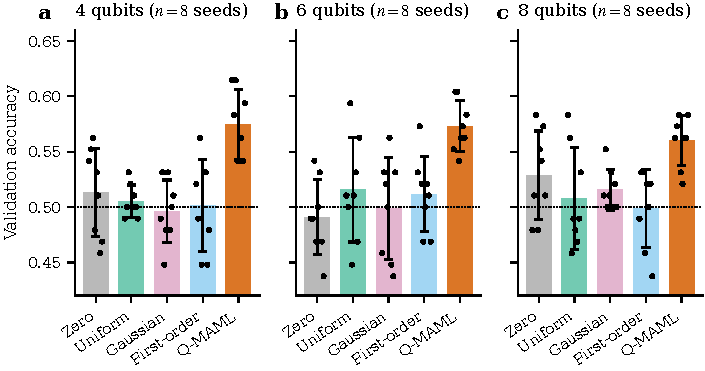
\includegraphics[width=\textwidth]{figures/fig_higgs.pdf}
\caption{\textbf{HIGGS classification.} Final validation accuracy by initialization (bars: mean; error bars: standard deviation; dots: individual seeds). Q-MAML is highest at 4, 6 and 8 qubits.}
\label{fig:higgs}
\end{figure}

\begin{table}[!htb]
\caption{\textbf{HIGGS validation accuracy} (mean $\pm$ s.d.\ over $n$ seeds), and Welch's $p$ (Cohen's $d$) for Q-MAML against Gaussian and against the post-hoc best classical scheme (uncorrected).}\label{tab:higgs}
\begin{tabular}{@{}lccc@{}}
\toprule
& 4 qubits & 6 qubits & 8 qubits \\
\midrule
Seeds ($n$) & 8 & 8 & 8 \\
\midrule
Zero & 0.513\,$\pm$\,0.040 & 0.491\,$\pm$\,0.034 & 0.529\,$\pm$\,0.040 \\
Uniform & 0.505\,$\pm$\,0.015 & 0.516\,$\pm$\,0.047 & 0.508\,$\pm$\,0.046 \\
Gaussian & 0.496\,$\pm$\,0.028 & 0.499\,$\pm$\,0.046 & 0.516\,$\pm$\,0.018 \\
First-order variant & 0.501\,$\pm$\,0.042 & 0.512\,$\pm$\,0.034 & 0.499\,$\pm$\,0.035 \\
\textbf{Q-MAML} & \textbf{0.574\,$\pm$\,0.032} & \textbf{0.573\,$\pm$\,0.023} & \textbf{0.560\,$\pm$\,0.023} \\
\midrule
Welch $p$ ($d$), Q-MAML vs Gaussian & $<0.001$ (2.6) & 0.002 (2.1) & $<0.001$ (2.1) \\
Welch $p$ ($d$), vs best classical & 0.005 (1.7; Zero) & 0.011 (1.5; Uniform) & 0.081 (1.0; Zero) \\
\botrule
\end{tabular}

\end{table}

Classification cost functions are also far more plateau-prone than the VQE costs: the gradient variance decays by $\sim$8 orders of magnitude from 4 to 10 qubits for every initialization, to a common floor, consistent with cross-entropy behaving as a global cost~\cite{cerezo2021costfunction}, whereas the Heisenberg VQE cost shows no exponential decay over 4--10 qubits at depth 3. Q-MAML does not change the scaling exponent in either domain (Section~\ref{sec:landscape}).

\subsection{Ten Hamiltonians}\label{sec:ten}

Table~\ref{tab:tracks} and Fig.~\ref{fig:scoreboard} summarize the ten systems at their base sizes. Two systems are consistent wins: the Schwinger model at $L{=}2$ (Q-MAML $0.18\%$ against $\pi$'s $0.22\%$; two wins and a tie), and SU(2) gauge theory at $N{=}2$, the largest margin observed, where Q-MAML reaches $\sim10^{-7}$ relative error at every seed against $10^{-4}$ for the best classical scheme, a $10^{3}\times$ margin. Neutrino oscillations ($N{=}4$) and supersymmetric quantum mechanics are wins at two of three seeds and a loss at the third, so the sign of the result is seed-dependent. Four systems are ties: the $\phi^4$ scalar field (Q-MAML $6.05\%$, Zero $6.12\%$; in the single-seed convergence curves Q-MAML reaches this value about three times sooner), light nuclei (all five schemes agree within 0.03\% at every seed, so the UCCSD ansatz makes the initial point irrelevant to the final energy, while Q-MAML alone avoids a shared oscillatory transient), scalar Yukawa (Q-MAML and Zero tie at the precision floor; the task range is near-vacuum, where Zero already starts close), and the Lipkin--Meshkov--Glick model (all schemes at or near the precision floor, and still at $J{=}3.5$, so Hilbert-space size alone does not make it discriminating). The $\mathbb{D}_8$ theory is a tie to slight loss against Uniform and Gaussian. Finally, $\mathbb{Z}_2$ gauge theory with a Gauss-law penalty is a loss at every seed; Section~\ref{sec:gauge} shows this is a property of the ansatz.

\begin{table}[!htb]
\caption{\textbf{Ten Hamiltonians at base size} ($n=3$ seeds): mean final relative error of Q-MAML and of the best classical scheme (best mean), and per-seed wins/ties/losses of Q-MAML against the best classical scheme at each seed (10\% tolerance; both below $10^{-6}$ counts as a tie). Track F is in log-gap because its ground energies are $\approx0$.}\label{tab:tracks}
\begin{tabular}{@{}llccc@{}}
\toprule
Track & System & Q-MAML error (\%) & Best classical (\%) & W/T/L \\
\midrule
A & Schwinger, $L{=}2$ & 0.181 & 0.216 ($\pi$) & 2/1/0 \\
B & $\mathbb{Z}_2$ LGT, penalty ansatz & 49.4 & 19.4 (Gaussian) & 0/0/3 \\
B & $\mathbb{Z}_2$ LGT, gauge-inv.\ ansatz & $2.2\!\times\!10^{-3}$ & 0.011 (Zero) & 3/0/0 \\
C & $\phi^4$ scalar field & 6.05 & 6.12 (Zero) & 0/3/0 \\
D & SU(2) LGT, $N{=}2$ & $1.3\!\times\!10^{-5}$ & 0.013 (Gaussian) & 3/0/0 \\
E & Neutrinos, $N{=}4$ & $3.6\!\times\!10^{-3}$ & $2.1\!\times\!10^{-3}$ ($\pi$) & 2/0/1 \\
F & SUSY QM & -4.48 (log-gap) & -4.75 (Uniform) & 2/0/1 \\
G & $\mathbb{D}_8$ LGT & 10.8 & 10.7 (Uniform) & 0/1/2 \\
H & Light nuclei (UCCSD) & 1.44 & 1.44 (Gaussian) & 0/3/0 \\
I & Scalar Yukawa & $2.7\!\times\!10^{-5}$ & $2.7\!\times\!10^{-5}$ (Zero) & 0/3/0 \\
J & LMG, $J{=}3/2$ & $2.7\!\times\!10^{-6}$ & $1.7\!\times\!10^{-6}$ (Zero) & 0/3/0 \\
\botrule
\end{tabular}

\end{table}

\begin{figure}[!htb]
\centering
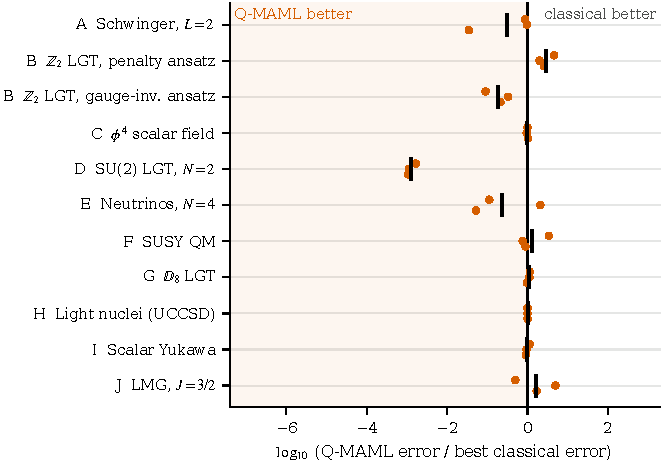
\includegraphics[width=0.78\textwidth]{figures/fig_scoreboard.pdf}
\caption{\textbf{Q-MAML against the best classical initialization, per seed.} Each dot is one seed (Q-MAML error divided by the best classical scheme's error at that seed, log scale); black ticks are seed means. Left of zero, Q-MAML is better. Track B is shown with both ansatze (Section~\ref{sec:gauge}).}
\label{fig:scoreboard}
\end{figure}

\begin{figure}[!htb]
\centering
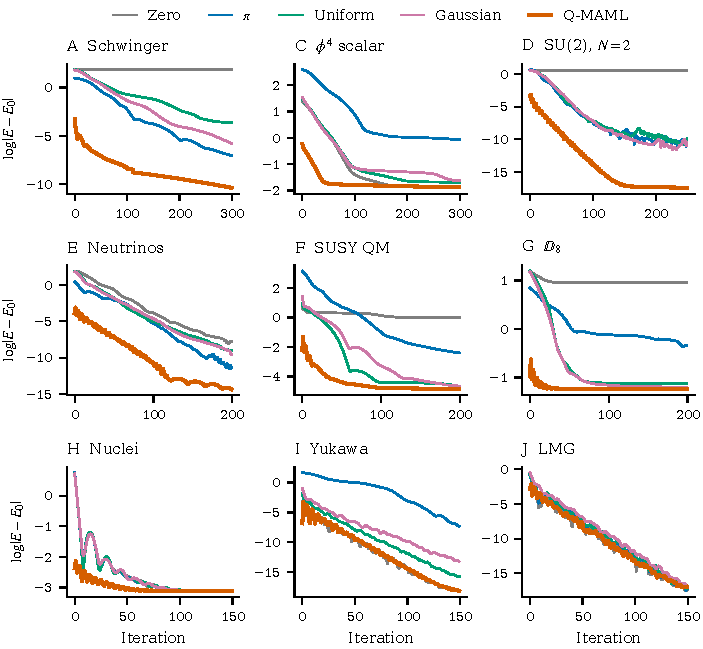
\includegraphics[width=\textwidth]{figures/fig_traj.pdf}
\caption{\textbf{Adaptation trajectories.} Mean log-gap to the ground energy over held-out tasks, by initialization, for the nine base-size systems not shown in Fig.~\ref{fig:calibration}. Track B is shown separately in Fig.~\ref{fig:gauge}.}
\label{fig:traj}
\end{figure}

\subsection{Structural gauge invariance decides the $\mathbb{Z}_2$ result}\label{sec:gauge}

With Gauss's law enforced by an energy penalty $V\sum_l(G_l-q_l)^2$ ($V{=}10$) on a hardware-efficient ansatz, Q-MAML loses to the best classical scheme at every one of three seeds ($49.4\pm13.7\%$ against $19.4\%$ for Gaussian, the best classical mean) with a nearly flat adaptation curve. A sweep over the penalty strength $V\in\{1,3,10,30\}$ refuted the obvious explanation that a large penalty drowns the task signal: Q-MAML is behind the best classical scheme at every $V$ tested, tying it only at the weakest ($V{=}1$). Two further experiments isolate the cause (Fig.~\ref{fig:gauge}). Replacing the ansatz with a gauge-invariant Hamiltonian-variational ansatz, whose layers Trotterize the physical Hamiltonian's own terms so that gauge invariance is structural, makes Q-MAML the best scheme at all three seeds, $3\times$--$10\times$ ahead of the best classical scheme ($0.0022\pm0.0011\%$ against $0.011\%$). A second ansatz of similar cost that is \emph{not} gauge-invariant leaves Q-MAML at or behind Uniform and Gaussian. Annealing the penalty during pretraining (Fig.~\ref{fig:gauge}b) roughly halves Q-MAML's mean error on the original ansatz ($49\%\to22$--$32\%$) but beats every classical scheme in only one of six seed--schedule cells. The final pretraining loss tracks the outcome: at $V{=}10$ the ground energies are $\approx+74.5$ (a penalty offset), the gauge-invariant Learner ends at the ground energy ($74.6$), and the annealed hardware-efficient Learners end $5$ or $25$--$27$ above it. These three comparisons use a reduced 4-task, 200-iteration budget; at the full 6-task, 300-iteration budget used everywhere else, the gauge-invariant ansatz replicates ($1.4\times10^{-5}$ against $4.3\times10^{-5}$ for the best classical scheme, a win at all three seeds, $2.5$--$6\times$ ahead) and the control ansatz is a loss at two of three seeds and a tie at the third. The two ansatze are different published circuits rather than a minimal pair, so the best-supported reading is that structural, not penalty-enforced, gauge invariance is what lets a learned initialization work; it is not a controlled ablation.

\begin{figure}[!htb]
\centering
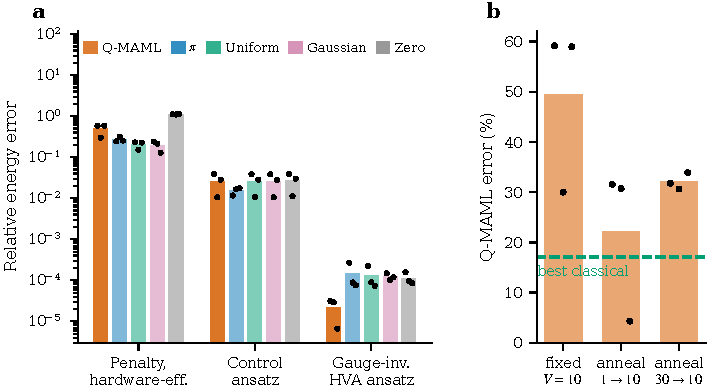
\includegraphics[width=\textwidth]{figures/fig_gauge.pdf}
\caption{\textbf{$\mathbb{Z}_2$ gauge theory: the ansatz decides.} \textbf{a}, Relative error for each scheme (bars: mean; dots: seeds) on the penalty-enforced hardware-efficient ansatz, a control ansatz that is not gauge-invariant, and the gauge-invariant ansatz. \textbf{b}, Q-MAML error with the penalty fixed or annealed during pretraining, against the best classical scheme (dashed).}
\label{fig:gauge}
\end{figure}

\subsection{Behavior with system size}\label{sec:scaling}

We extended three systems to larger sizes, verifying each Hamiltonian first (Fig.~\ref{fig:scaling}). For neutrino oscillations the win strengthens: at $N{=}6$ Q-MAML is best at all three seeds, $135\times$, $\approx77\times$ and $144\times$ ahead of $\pi$, the best classical scheme. For SU(2) gauge theory the $N{=}2$ advantage does not carry over. At $N{=}3$ a converging budget (depth 6) puts $\pi$ first at every seed ($0.28\pm0.07\%$) with Q-MAML a stable second ($2.02\pm0.39\%$); at $N{=}4$ Q-MAML becomes seed-unstable, at $23.3\%$, $2.9\%$ and $450\%$ across three seeds while $\pi$ holds at $3.5$--$6.0\%$. (An earlier depth-4 run at $N{=}3$ showed every scheme failing at 200--500\%, a budget artifact.) For the Schwinger model the original $L{=}4$ (8-qubit) run failed, with Q-MAML at $31.8\%$ against $\pi$'s $8.6\%$.

\begin{figure}[!htb]
\centering
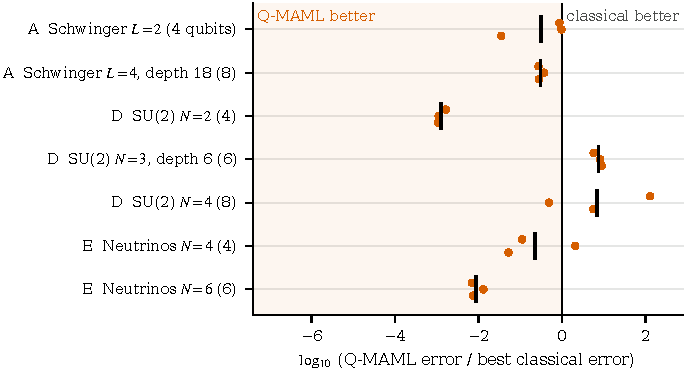
\includegraphics[width=0.78\textwidth]{figures/fig_scaling.pdf}
\caption{\textbf{Larger systems.} As in Fig.~\ref{fig:scoreboard}, for each system size (qubits in parentheses). The neutrino win strengthens with size; the SU(2) advantage at $N{=}2$ is replaced by a tie or loss and, at $N{=}4$, seed instability. The Schwinger $L{=}4$ point uses a lighter protocol (3 tasks, 150 iterations).}
\label{fig:scaling}
\end{figure}

\paragraph{Why Q-MAML fails at larger sizes.} For SU(2) $N{=}4$ we recorded the full pretraining history and per-task energies before and after adaptation for three seeds and two pretraining settings (Fig.~\ref{fig:diag}a,b). The three seeds are three different regimes. At seed 1 both settings converge to the same good solution (training meta-loss $-0.27$, initial energies within $\sim$0.2 of the ground energies), and the adapted energies agree to $10^{-4}$ or better. At seed 2 both converge to the same bad one: the meta-loss stalls near $0.95$ against ground energies of $\approx-0.3$, and adaptation cannot move the initialization at all (final equals initial energy to two digits), so the predicted point is effectively a stationary point of each task's cost. At seed 0 the original setting diverges (the meta-loss rises) and a lower learning rate stalls on an intermediate plateau. A lower learning rate and more epochs, the fix that repaired the Schwinger $L{=}4$ pretraining, therefore does not repair these seeds. Two consequences follow: ``pretraining converged'' is not ``pretraining worked'', and the failure is visible in the training meta-loss without any test data. We tested the second consequence directly: six Learner initializations were pretrained per data seed at the original $N{=}4$ setting and scored by held-out error against final training loss (Fig.~\ref{fig:diag}c). A final loss near the mean ground energy ($\approx-0.3$) was always followed by a low error (five of five restarts, $2.0$--$3.4\%$, at or below $\pi$); a stalled loss ($\gtrsim1$) was a warning but not a reliable one, since one data seed's stalled restarts spanned $2.0$--$15.1\%$. Selecting the restart with the lowest training loss beat $\pi$ at both data seeds tested ($2.3\%$ and $2.0\%$ against $3.5\%$ and $4.2\%$), turning the diagnostic into a usable selection rule. The Schwinger model at $L{=}4$ behaves differently. A lower pretraining learning rate repairs pretraining (mean energy inside the range of the true ground energies) but at depth 12 the adapted result stays mixed across seeds ($21.2\%$ against $\pi$'s $17.9\%$ at seed 0; $20.4\%$ against $25.0\%$ at seed 1), whereas depth 18 gives Q-MAML the lead at every seed run (Fig.~\ref{fig:scaling}), even at the original learning rate where pretraining still stalls (seed 0: $4.5\%$ against $8.7\%$). Depth, not pretraining convergence, is the operative variable there; whether a stalled-pretraining Learner still contributes beyond a small-angle start was not isolated.

\begin{figure}[!htb]
\centering
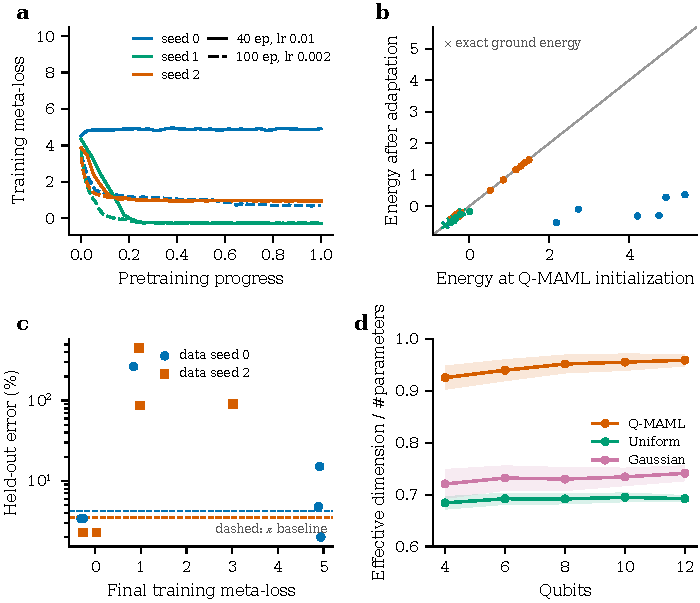
\includegraphics[width=\textwidth]{figures/fig_diag.pdf}
\caption{\textbf{Mechanisms.} \textbf{a}, SU(2) $N{=}4$ training meta-loss for three seeds and two pretraining settings: seed 1 converges to a good solution, seed 2 to a poor one, seed 0 diverges at the original setting. \textbf{b}, Energy at Q-MAML's initialization against energy after adaptation, per test task (crosses: exact ground energies): at seed 2 points lie on the diagonal (adaptation cannot move them), far above the ground energies. \textbf{c}, Held-out error against final training loss for six Learner restarts at each of two data seeds; dashed lines are the $\pi$ baseline. \textbf{d}, Effective dimension of the quantum Fisher information matrix at initialization (Heisenberg XYZ ansatz, 20 samples per point; shading: s.d.).}
\label{fig:diag}
\end{figure}

\subsection{Placement in parameter space, not plateau resistance}\label{sec:landscape}

A McClean-style scan of the gradient variance at a reference parameter shows Q-MAML's variance comparable to or larger than the classical schemes' at every qubit count from 4 to 14 and no change in the scaling exponent, so Q-MAML is not resisting barren plateaus. A single-coordinate gradient cannot distinguish a circuit that is degenerate everywhere from one degenerate along a few directions, so we also computed the quantum Fisher information matrix (block-diagonal metric tensor) at each sampled initialization and summarized it by the participation ratio of its spectrum, normalized by the number of parameters, an effective dimension (Fig.~\ref{fig:diag}d). Q-MAML initializations have consistently higher effective dimension ($0.925\pm0.022$ at 4 qubits rising to $0.959\pm0.011$ at 12) than Uniform ($0.684$--$0.695$) or Gaussian ($0.721$--$0.741$), and the gap does not shrink with qubit number. This gives quantitative form to the intuition that Q-MAML's benefit lies in where it places the circuit in parameter space; it measures local effective dimension at the initialization, on one ansatz, not whether that translates into faster adaptation.

%% =====================================================================================
\section{Discussion}\label{sec:discussion}

The results do not support a blanket claim that learned initialization helps HEP simulations; they support a conditional one. It helps where a task-dependent good region exists and pretraining can find it: small systems with structurally symmetric ansatze (Schwinger $L{=}2$, SU(2) $N{=}2$, gauge-invariant $\mathbb{Z}_2$), and neutrino oscillations up to six qubits. It is unnecessary where the initial point does not matter (UCCSD nuclei), where a trivial initialization is already near the answer (near-vacuum Yukawa) or where the benchmark is too easy to discriminate (LMG). And it is unreliable where the meta-objective has poor local minima that pretraining finds (SU(2) $N{=}4$). Two practical recommendations follow. Compare against $\pi$ and Uniform, since no classical scheme is a safe default ($\pi$ is best at some systems and worst at others) and the $\pi$ baseline was best or tied for best at several sizes. And monitor the training meta-loss against the (cheap, classically computed) mean ground energy of the training tasks: when several Learner initializations are pretrained, the one with the lowest final loss is a usable selection rule, since it recovered a win over $\pi$ at SU(2) $N{=}4$ without test data.

\paragraph{Limitations.} The largest system is 12 qubits (the Fisher probe) and typically 4--8; all results are noiseless simulation of interpolation over a task range, and we do not test extrapolation across a phase transition beyond one scalar-field experiment where Q-MAML did not generalize. Three seeds resolve large effects but not small ones, and several extensions (neutrino $N{=}6$ excepted) and mechanism experiments use a reduced budget or a single seed, as stated. Track-level results use a fixed hardware-efficient ansatz (except nuclei and the $\mathbb{Z}_2$ comparison), so they measure relative initialization quality on a given ansatz, not the best achievable VQE. We use the un-reduced SU(2) and $\mathbb{D}_8$ Hamiltonians, not the qubit-reduced constructions of their source papers. Track E and I are reformulations of real-time problems as ground-state problems. The SU(2) $N{=}4$ instability is diagnosed, not fixed.

%% =====================================================================================
\section{Conclusion}\label{sec:conclusion}

Q-MAML reproduces the original paper's 15--20$\times$ gains and improves HEP classification, but on lattice and field-theory Hamiltonians its benefit is conditional on ansatz structure and system size, and two apparent results reverse under scrutiny: a loss on $\mathbb{Z}_2$ gauge theory that is an artifact of the penalty-enforced ansatz, and an SU(2) advantage at four qubits that does not survive to eight. The most transferable findings are diagnostic: a failing initialization is visible in the training meta-loss and can be worked around by restarting and selecting on that loss, and a Fisher-information probe shows Q-MAML's gain is placement in parameter space, not resistance to plateaus. Natural next steps are larger systems and hardware noise, and the qubit-reduced formulations of the SU(2) and $\mathbb{D}_8$ theories.

\FloatBarrier
\backmatter

\bmhead{Acknowledgements}
[To be completed by the author.]

\section*{Declarations}
\begin{itemize}
\item \textbf{Funding:} [to be confirmed by the author]
\item \textbf{Competing interests:} [to be confirmed by the author]
\item \textbf{Data and code availability:} All code, notebooks and saved results are at [repository URL to be completed by the author]. The HIGGS dataset is public~\cite{baldi2014higgs}.
\item \textbf{Author contribution:} A.K.\ designed and ran all experiments and wrote the manuscript.
\end{itemize}

\begin{thebibliography}{99}
\bibitem{leeqmaml2025} Lee, J., Cho, J., Kim, S.: Q-MAML: Quantum model-agnostic meta-learning for variational quantum algorithms. In: Proc.\ AAAI, vol.\ 39, pp.\ 18137--18144 (2025). arXiv:2501.05906
\bibitem{cerveralierta2021metavqe} Cervera-Lierta, A., Kottmann, J.S., Aspuru-Guzik, A.: Meta-variational quantum eigensolver: learning energy profiles of parameterized Hamiltonians for quantum simulation. PRX Quantum \textbf{2}, 020329 (2021)
\bibitem{mcclean2018barren} McClean, J.R., Boixo, S., Smelyanskiy, V.N., Babbush, R., Neven, H.: Barren plateaus in quantum neural network training landscapes. Nat.\ Commun.\ \textbf{9}, 4812 (2018)
\bibitem{cerezo2021costfunction} Cerezo, M., Sone, A., Volkoff, T., Cincio, L., Coles, P.J.: Cost function dependent barren plateaus in shallow parametrized quantum circuits. Nat.\ Commun.\ \textbf{12}, 1791 (2021)
\bibitem{grant2019initialization} Grant, E., Wossnig, L., Ostaszewski, M., Benedetti, M.: An initialization strategy for addressing barren plateaus in parametrized quantum circuits. Quantum \textbf{3}, 214 (2019)
\bibitem{zhang2022escaping} Zhang, K., Liu, L., Hsieh, M.-H., Tao, D.: Escaping from the barren plateau via Gaussian initializations in deep variational quantum circuits. In: NeurIPS (2022)
\bibitem{wang2023trainability} Wang, X., et al.: Trainability enhancement of parameterized quantum circuits via reduced-domain parameter initialization. arXiv:2302.06858 (2023)
\bibitem{qracle2025} Zhang, C., Jiang, L., Chen, F.: Qracle: a graph-neural-network-based parameter initializer for variational quantum eigensolvers. arXiv:2505.01236 (2025)
\bibitem{diffq2025} Zhang, C., Zheng, M., Lou, Q., Chen, F.: DiffQ: parameter initialization for variational quantum algorithms via generative diffusion models. arXiv:2509.17324 (2025)
\bibitem{baldi2014higgs} Baldi, P., Sadowski, P., Whiteson, D.: Searching for exotic particles in high-energy physics with deep learning. Nat.\ Commun.\ \textbf{5}, 4308 (2014)
\bibitem{schwingertrappedion2025} Trapped-ion demonstration of variational quantum simulation of the interacting Schwinger model. arXiv:2504.20824 (2025) [author list to be completed]
\bibitem{z2lgtbp2025} Barren-plateau-free variational quantum simulation of $\mathbb{Z}_2$ lattice gauge theories. arXiv:2507.19203 (2025) [author list to be completed]
\bibitem{scalarfield2023} Li, A.C.Y., Macridin, A., Mrenna, S., Spentzouris, P.: Simulating scalar field theories on quantum computers with limited resources. arXiv:2210.07985 (2023)
\bibitem{su2hadrons2021} SU(2) hadrons on a quantum computer via a variational approach. Nat.\ Commun.\ \textbf{12}, 6499 (2021). arXiv:2102.08920 [author list to be completed]
\bibitem{neutrinoqc2021} Simulating collective neutrino oscillations on a quantum computer. arXiv:2102.12556 (2021) [author list to be completed]
\bibitem{duanfullerqian2010} Duan, H., Fuller, G.M., Qian, Y.-Z.: Collective neutrino oscillations. Annu.\ Rev.\ Nucl.\ Part.\ Sci.\ \textbf{60}, 569--594 (2010)
\bibitem{susyqm2026} Simulating supersymmetric quantum mechanics with variational quantum algorithms. arXiv:2603.18749 (2026) [author list to be completed]
\bibitem{d8lgt2025} Gaz, E., Popov, P.P., Pardo, G., Lewenstein, M., Hauke, P., Zohar, E.: Quantum simulation of non-Abelian lattice gauge theories: a variational approach to $\mathbb{D}_8$. arXiv:2501.17863 (2025)
\bibitem{nucleareft2026} Cifci, P., Akkoyun, S., La Ronde, L.: Systematic VQE benchmarking of the deuteron, triton, and helium-3 within lattice pionless effective field theory. arXiv:2604.20908 (2026)
\bibitem{yukawa2022} Kaldenbach, T.N., Heller, M., Alber, G., Stojanovic, V.M.: Digital quantum simulation of scalar Yukawa coupling. arXiv:2211.02684 (2022)
\bibitem{hlvqe2023} Robin, C.E.P., Savage, M.J.: Quantum simulations in effective model spaces (I): Hamiltonian-learning VQE using digital quantum computers and application to the Lipkin--Meshkov--Glick model. Phys.\ Rev.\ C \textbf{108}, 024313 (2023)
\end{thebibliography}
